\subsubsection{\stid{3.01} xSDK4ECP} 
\paragraph{Overview} The xSDK4ECP project is creating a value-added aggregation of DOE math and scientific libraries through the {\em xSDK} (Extreme-scale Scientific Software Development Kit)~\cite{xsdk:homepage}, which increases the combined usability, standardization, and interoperability of these libraries as needed by ECP. The project focuses on community development and a commitment to combined success via quality improvement policies, better build infrastructure, and the ability to use diverse, independently developed xSDK libraries in combination to solve large-scale multiphysics and multiscale problems.  We are extending draft xSDK package community policies and developing interoperability layers among numerical libraries in order to improve code quality, access, usability, interoperability, and sustainability. Focus areas are (1) coordinated use of on-node resources, (2) integrated execution (control inversion and adaptive execution strategies), and (3) coordinated and sustainable documentation, testing, packaging, and deployment. Starting FY20, the project will also investigate and deploy multiprecision functionality in the ECP ST ecosystem to enable the use of low-precision hardware function units, reduce the pressure on memory and communication interfaces and achieve improved performance.

xSDK4ECP is needed for ECP because it enables ECP apps such as ExaAM and ExaWind to seamlessly leverage the entire scientific libraries ecosystem.  For example, ExaWind has extremely challenging linear solver scaling problems.  xSDK4ECP provides access to all scalable linear solvers with minimal changes.  xSDK4ECP is also an essential element of the product release process for ECP ST.  xSDK4ECP provides an aggregate build and install capability for all ECP math libraries that supports hierarchical, modular installation of ECP software.  Finally, xSDK4ECP provides a forum for collaborative math library development, helping independent teams to accelerate adoption of best practices, enabling interoperability of independently developed libraries and improving developer productivity and sustainability of the ECP ST software product.

\paragraph{Key Challenges}
The complexity of application codes is steadily increasing due to more sophisticated scientific models.  While some application areas will use Exascale platforms for higher fidelity, many are using the extra computing capability for increased coupling of scales and physics.  Without coordination, this situation  leads to difficulties when building application codes that use 8 or 10 different libraries, which in turn might require additional libraries or even different versions of the same libraries.

The xSDK represents a different approach to coordinating library development and deployment.  Prior to the xSDK, scientific software packages were cohesive with a single team effort, but not across these efforts. The xSDK goes a step further by developing community policies followed by each independent library included in the xSDK.  This policy-driven, coordinated approach enables independent development that still results in compatible and composable capabilities.

\paragraph{Solution Strategy}

The xSDK effort has two primary thrusts:
\begin{enumerate}
	\item \textbf{Increased interoperability:} xSDK packages can be built with a single Spack package target.  Furthermore, services from one package are accessible to another package.
	\item \textbf{Increased use of common best practices:}  The xSDK has a collection of community policies that set expectations for a package, from best design practices to common look-and-feel.
\end{enumerate}

xSDK interoperability efforts began first with eliminating incompatibilities that prohibited correct compilation and integration of the independently developed libraries.  These issues include being able to use a common version of a library such as SuperLU by PETSc and Trilinos.  The second, and ongoing phase is increased use of one package's capabilities from another.  For example, users who build data objects using PETSc can now access Trilinos solvers without copying to Trilinos data structures. xSDK community package policies~\cite{xsdk-policies:homepage,xSDK-community-package-policies2019} are a set of minimum requirements (including topics of configuring, installing, testing, MPI usage, portability, contact and version information, open source licensing, namespacing, and repository access) that a software package must satisfy in order to be considered xSDK compatible. The designation of xSDK compatibility informs potential users that a package can be easily used with others. 
xSDK community installation policies~\cite{xSDK-community-installation-policies2019} help make configuration and installation of xSDK software and other HPC packages as efficient as possible on common platforms, including standard Linux distributions and Mac OS X, as well as on target machines currently available at DOE computing facilities (ALCF, NERSC, and OLCF) and eventually on new Exascale platforms.
Community policies for the xSDK promote long-term sustainability and interoperability among packages, as a foundation for supporting complex multiphysics and multiscale ECP applications. In addition, because new xSDK packages will follow the same standard, installation software and package managers (for example, Spack~\cite{gamblin+:sc15}) can easily be extended to install many packages automatically.

For the adaptive execution effort, the team is working towards GPTune, a Gaussian process tuner, to help math library users to find the optimal parameter settings for the libraries to achieve high performance for their applications. In addition, an interface will be created to also give access to alternate autotuners.
Regarding the multiprecision effort, the project will assess current status and functionalities, advance the theoretical knowledge on multiprecision algorithms, design prototype implementations and multiprecision interoperability layers, deploy production-ready multiprecision algorithms in the xSDK math libraries, ensure multiprecision cross-library interoperability and integrate multiprecision algorithms into ECP application projects.

\paragraph{Recent Progress}

Figure~\ref{fig:xsdk-schematic} illustrates a new {\em Multiphysics
	Application C}, built from two complementary applications that can
readily employ any libraries in the xSDK, shown in green.  Current xSDK member packages (xSDK-0.5.0, released November 2019) are the four founding libraries
(hypre~\cite{hypre:homepage}, PETSc~\cite{petsc:homepage}, SuperLU~\cite{superlu:homepage}, and Trilinos~\cite{trilinos:homepage}), three libraries added in xSDK-0.3.0, released December 2017 (MAGMA~\cite{magma:homepage}, MFEM~\cite{mfem:homepage}, and SUNDIALS~\cite{sundials:homepage}), and ten more libraries added xSDK-0.4.0, released in December 2018, including seven with DOE support (AMRex~\cite{amrex:homepage}, DTK~\cite{dtk:homepage}, Omega\_h~\cite{omega_h:homepage}, PLASMA~\cite{plasma:homepage}, PUMI~\cite{pumi:homepage}, STRUMPACK~\cite{strumpack:homepage}, and Tasmanian~\cite{tasmanian:homepage}) and three in the broader community (deal.II~\cite{deal.ii:homepage}, PHIST~\cite{phist:homepage}, and SLEPc~\cite{slepc:homepage}), and four new xSDK members libEnsemble~\cite{libensemble:homepage}, Ginkgo~\cite{ginkgo:homepage}, preCICE~\cite{precice:homepage}, and ButterflyPACK~\cite{butterflypack:homepage}.
Application domain components are represented
in orange.  Of particular note is Alquimia~\cite{alquimia:homepage}, a domain-specific interface
that support uniform access to multiple biogeochemistry capabilities, including
PFLOTRAN~\cite{pflotran:homepage}.  Additional libraries have announced their interest in working toward becoming xSDK member packages and participating in future xSDK releases.
\begin{figure}[htb]
	\centering
	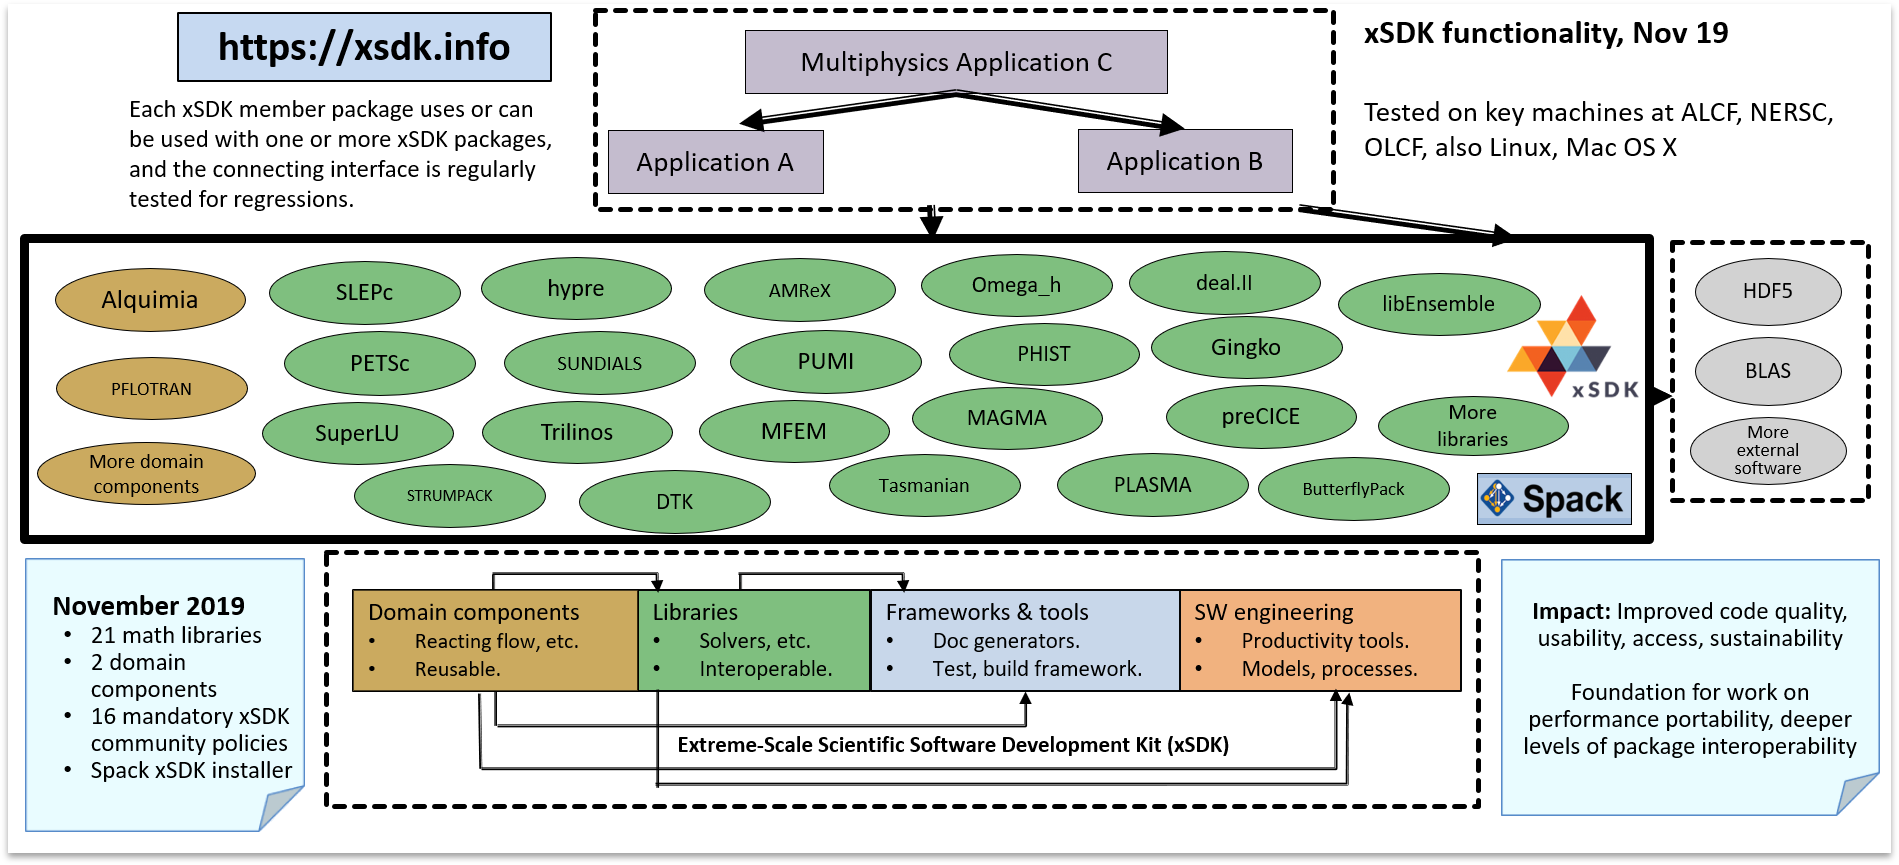
\includegraphics[width=5in]{projects/2.3.3-MathLibs/2.3.3.01-xSDK/xSDK-diagram.png}
	\caption{\label{fig:xsdk-schematic} The above diagram shows how multiphysics and multiscale applications can readily access xSDK packages.}
\end{figure}

% The arrows among the xSDK libraries indicate current support for
% a package to call another to provide scalable linear solvers
% functionality on its behalf.  For example, {\em Application~A} could
% use PETSc for an implicit-explicit time advance, which in turn could
% interface to SuperLU to solve the resulting linear systems with a
% sparse direct solver.  {\em Application~B} could use Trilinos to solve
% a nonlinear system, which in turn could interface to hypre to solve
% the resulting linear systems with algebraic multigrid.  Of course,
% many other combinations of solver interoperability are also possible.
%Each xSDK member package uses or can be used with one or more xSDK packages, and the connecting interface is regularly tested for regressions.  
%The sites \url{https://xsdk.info/example-usage} and \cite{Klinvex-xSDKTrilinos} provide examples of xSDK usage, including interoperability among linear solvers in hypre, PETSc, SuperLU, and Trilinos.
The xSDK team also continued development of the community policies with a new release 0.5.0. The policies were updated, and a new recommended policy was added with feedback from the ECP community. The policies were moved to github, and the process on changing or proposing policies has been updated.

\paragraph{Next Steps}

Our next efforts include the incorporation of more libraries and the extension of application usage to evaluate the effectiveness of current functionality and to motivate new capabilities. Regarding autotuning of code performance, we will finish a prototype autotuning framework using the multi-output Gaussian process ML approach which includes multitask and transfer learning. The xSDK4ECP team will also investigate the use of multiprecision for math libraries and document the results of the investigation.
%\begin{enumerate}
%	\item \textbf{Include more libraries:} xSDK4ECP will continue efforts to expand the number of participating packages, adapt community policies, and exploit increased interoperability.  We are coordinating with broader SDK efforts and working toward the inclusion of additional domain application packages.
%	\item \textbf{Extend application usage:}  xSDK4ECP will continue partnering with application teams to evaluate the effectivness of current functionality and to motivate new capabilities.
%	\item \textbf{Autotuning of code performance:} The team will finish a prototype autotuning framework using the multi-output Gaussian Process ML approach which includes multitask and transfer learning.
%	\item \textbf{Multiprecision effort:} The xSDK4ECP team will investigate the use of multiprecision for the math libraries and document the results of the investigation. 

% 		\item \textbf{Process control transfer interfaces:} The ever-increasing use of concurrency within the top-level MPI processes requires that computational resources used by an application or library can be transferred to another library. Transfer of these resources is essential for obtaining good performance.  The xSDK project will develop interfaces to support sharing and transfer of computational resources.	
%\end{enumerate}
